\documentclass[11pt]{article}

% ── Packages ──────────────────────────────────────────────────────────
\usepackage[T1]{fontenc}
\usepackage[margin=2.5cm]{geometry}
\usepackage{lmodern}
\usepackage{amsmath,amssymb,amsthm,mathtools}
\usepackage{array,tabularx}
\usepackage{booktabs}
\usepackage{graphicx}
\usepackage[final]{microtype}
\usepackage{hyperref}
\usepackage{cleveref}
\usepackage{algorithm}
\usepackage{algpseudocode}
\usepackage{tikz}
\usetikzlibrary{arrows.meta,positioning,calc,decorations.pathreplacing}
\usepackage{subcaption}
\usepackage{xcolor}
\usepackage{enumitem}

% ── Theorem environments ──────────────────────────────────────────────
\theoremstyle{definition}
\newtheorem{definition}{Definition}[section]
\theoremstyle{plain}
\newtheorem{theorem}[definition]{Theorem}
\newtheorem{lemma}[definition]{Lemma}
\newtheorem{proposition}[definition]{Proposition}
\newtheorem{conjecture}[definition]{Conjecture}
\theoremstyle{remark}
\newtheorem{remark}[definition]{Remark}
\newtheorem{invariant}[definition]{Invariant}

% ── Custom commands ───────────────────────────────────────────────────
\newcommand{\Ostr}{\mathcal{O}}          % Order strength
\newcommand{\Clvl}{\mathcal{C}}          % Closure level
\newcommand{\Cdep}{\mathcal{C}_{\mathrm{dep}}}
\newcommand{\Ccoh}{\mathcal{C}_{\mathrm{coh}}}
\newcommand{\Cfr}{\mathcal{C}_{\mathrm{fr}}}
\newcommand{\Ffin}{\mathcal{F}}          % Finality function
\newcommand{\Uord}{U_{\mathrm{order}}}   % Order utility
\newcommand{\Rcls}{R_{\mathrm{closure}}} % Closure risk
\newcommand{\Frag}{\mathrm{FragilityCoupling}}
\newcommand{\Phifn}{\Phi}               % Bi-objective functional
\newcommand{\Dag}{\mathcal{G}}          % DAG graph
\newcommand{\Rset}{\mathbb{R}}          % Reals
\newcolumntype{L}[1]{>{\raggedright\arraybackslash}p{#1}}
\newcolumntype{Y}{>{\raggedright\arraybackslash}X}
\newcommand{\codepath}[1]{\path{#1}}

\definecolor{blueblock}{RGB}{70,130,180}
\definecolor{redblock}{RGB}{205,92,92}
\definecolor{closurecolor}{RGB}{60,150,80}

% ── Typography and float tuning ───────────────────────────────────────
\linespread{1.03}
\allowdisplaybreaks[2]
\setlength{\emergencystretch}{2em}
\setlength{\textfloatsep}{14pt plus 2pt minus 4pt}
\setlength{\floatsep}{12pt plus 2pt minus 2pt}
\setlength{\intextsep}{12pt plus 2pt minus 2pt}
\captionsetup{font=small,labelfont=bf,skip=6pt}
\setlist[itemize,enumerate,description]{topsep=4pt,itemsep=2pt,parsep=0pt,partopsep=0pt}
\urlstyle{same}
\raggedbottom

% ── Metadata ──────────────────────────────────────────────────────────
\title{\textbf{PHASMDAG: Bi-Objective, Closure-Aware DAG Consensus}\\[6pt]
{\large Towards a Separation of Order, Closure, and Finality\\
in High-Throughput Proof-of-Work Consensus}}
\author{Arthur Zhang}
\date{April 2026}

\begin{document}
\maketitle

% =====================================================================
\begin{abstract}
This paper sets out a preliminary formulation of \emph{PHASMDAG}, a
bi-objective, closure-aware DAG consensus protocol intended to separate three
semantic roles that remain conflated in existing GhostDAG-family designs:
\emph{ordering}, \emph{closure maturity}, and \emph{finality}.
Recent work by Wu, Wei, Zhang, and Jiang\,(NDSS\,2024) suggests that the
\emph{Decoupling Assumption}---a prerequisite for the security analyses of the
major DAG-based PoW protocols---may fail under sufficiently high throughput,
owing to Block Jam and Late-Predecessor effects.
The present paper proceeds from the contention that the underlying difficulty
in GhostDAG-family protocols may lie not only in the vulnerability of relay
paths, but also in the demand placed upon a single structural classifier to
stand simultaneously for canonical order, safe acceptability, and finality
confidence.
PHASMDAG accordingly treats closure as a first-class protocol state and studies
a bi-objective consensus functional
$\Phifn(S) = \Uord(S) - \lambda\,\Rcls(S)$
that trades structural concurrency against dependency fragility.
In the proposed $v_0$ instantiation, the closure layer is expressed through
three deterministic sub-metrics---dependency completeness, descendant-support
coherence, and frontier stability---whose aggregation and penalty terms are
rendered protocol-visible.
The paper develops this protocol sketch, records a preliminary security
heuristic under the Congestible Blockchain Model, and isolates
\emph{closure coherence} as the principal unresolved theorem target for any
consistent notion of strong confirmation.
\end{abstract}

\noindent{\small\textbf{Keywords:} DAG consensus; GhostDAG; closure-aware consensus;
late predecessor; block jam; bi-objective optimisation; finality semantics}

% =====================================================================
\section{Introduction}\label{sec:intro}

DAG-based Proof-of-Work consensus protocols---SPECTRE~\cite{sompolinsky2016spectre},
PHANTOM/GhostDAG~\cite{sompolinsky2018phantom,sompolinsky2021ghostdag},
OHIE~\cite{yu2021ohie}, and Prism~\cite{bagaria2019prism}---represent the most
promising direction for scaling Nakamoto consensus beyond the throughput ceiling
imposed by chain-style protocols.
By allowing blocks to reference multiple parents and thereby capture concurrency,
these protocols achieve block rates that far exceed the network delay bound $D$.

However, Wu et al.~\cite{wu2024security} proved that this performance gain comes
with a previously unaccounted security cost.
Their \emph{Congestible Blockchain Model}\,(CBM) shows that when block production
rate $f$ is high relative to network capacity, two phenomena emerge:
\begin{enumerate}[nosep]
    \item \textbf{Block Jam}\,(BJ): when the total size of priority blocks in a
    time window exceeds the network's relay capacity, these blocks cannot
    propagate within the assumed delay~$D$.
    \item \textbf{Late Predecessor}\,(LP): a block's propagation completion does
    not imply its acceptability---a block can only be accepted after \emph{all}
    its predecessors have been received and validated.
    If a predecessor arrives later than its successor, the successor's actual
    delay ($\Delta_{\mathrm{actual}} = \Delta_{\mathrm{prop}} +
    \Delta_{\mathrm{proc}}$) exceeds its propagation delay alone.
\end{enumerate}

Together, BJ and LP violate the \emph{Decoupling
Assumption}~\cite{wu2024security}: the assumption that priority blocks can
propagate within fixed short delay $D$ \emph{and} be immediately accepted and
built upon.  All existing security proofs for DAG-based PoW protocols rely on
this assumption.

\paragraph{Contribution summary.}
\begin{enumerate}[nosep]
    \item \textbf{Root-cause diagnosis.}
    It is argued that the fundamental limitation of GhostDAG-family protocols
    lies not merely in the attackability of relay paths, but in the requirement
    that a single structural classifier should simultaneously represent
    canonical order, safe acceptability, and finality confidence.
    This conflation is largely invisible under optimistic network assumptions,
    but becomes a security liability under CBM.

    \item \textbf{Protocol design.}
    A candidate protocol design is set out in which order, closure maturity,
    and finality are separated into three explicit semantic layers.
    The proposal introduces closure as a first-class protocol state together
    with a bi-objective consensus functional
    $\Phifn(S) = \Uord(S) - \lambda\,\Rcls(S)$ that penalises dependency
    fragility.
    For $v_0$, a GhostDAG-style blue-work lineage is taken as the canonical
    order core, while closure is instantiated through the deterministic
    sub-metrics $\Cdep(B)$, $\Ccoh(B)$, and $\Cfr(B)$.

    \item \textbf{Preliminary security analysis.}
    A preliminary closure-modulated chain-growth heuristic is recorded under the
    CBM, together with a candidate dominance region in which closure awareness
    may outperform purely structural finality under LP attack.
    Claims advanced here are explicitly separated from claims that remain to be
    established.

    \item \textbf{Formal modelling and verification roadmap.}
    A compositional formal model, a simulation-based evaluation methodology,
    and a phased verification programme are delineated around the theorem
    target of closure coherence.
\end{enumerate}

\paragraph{On the designation ``PHASM''.}
The designation \emph{PHASMDAG} is intended to evoke
\emph{phase-separated semantics}: order, closure, and finality are treated as
distinct protocol phases rather than being collapsed into a single structural
score.

\paragraph{Claim status.}
This document is intentionally written as a protocol proposal rather than as a
completed proof artifact.
\textbf{Definitions} specify protocol intent.
\textbf{Lemmas} and \textbf{Propositions} are preliminary and hold only under
the modelling assumptions stated around them.
\textbf{Conjectures} identify unresolved validation targets.
The most important unresolved target is \emph{closure coherence}: whether
$\Clvl(B)$ converges sufficiently across honest nodes to support consistent
strong confirmation.

% =====================================================================
\section{Related Work and Theoretical Context}\label{sec:background}

\subsection{Throughput, Security, and Delay in PoW Consensus}

The tension between throughput and network delay predates DAG-based consensus.
Sompolinsky and Zohar's high-rate Bitcoin analysis~\cite{sompolinsky2013secure}
already emphasised that short inter-block intervals and bounded delay cannot be
treated independently.
Formal longest-chain analyses subsequently made this dependence explicit
through common-prefix, chain-growth, and chain-quality style guarantees under
bounded-delay assumptions~\cite{garay2015backbone}.
Zhang and Preneel~\cite{zhang2019common} later unified these perspectives into
a common-metrics framework, making it possible to compare protocol families
under aligned security notions rather than under protocol-specific metrics.

Two considerations may be taken from that literature.
First, performance claims in PoW systems are meaningful only relative to an
explicit delay model.
Second, security arguments become fragile when propagation, acceptance, and
mining eligibility are silently conflated.

\subsection{DAG-Based PoW Ordering Protocols}

The DAG-based PoW literature can be organised by the manner in which
concurrency is converted into order:
\begin{description}[nosep]
    \item[SPECTRE~\cite{sompolinsky2016spectre}] provides fast confirmation
    through pairwise voting, but does not aim to maintain a global total order.

    \item[PHANTOM~\cite{sompolinsky2018phantom}] formulates ordering as a
    $k$-cluster identification problem, thereby making explicit the relation
    between concurrency and anticone structure.

    \item[GhostDAG~\cite{sompolinsky2021ghostdag}] replaces exact clustering
    with a greedy $K$-cluster approximation, yielding a practical structural
    order rule based on blue-set growth and blue-work accumulation.

    \item[OHIE~\cite{yu2021ohie}] separates transaction handling from
    structural ordering through a numbered-chain construction.

    \item[Prism~\cite{bagaria2019prism}] decomposes consensus into proposal,
    voting, and committee roles, thereby achieving high throughput through
    role separation rather than through a single ordering object.
\end{description}

The present paper differs from these systems in one principal respect.
The distinctive feature is not the use of a DAG per se, but the explicit
separation of \emph{order}, \emph{closure maturity}, and \emph{finality} as
distinct protocol-level semantic objects.

\subsection{Congestion, Delayed Acceptability, and Strategic Deviation}

Wu et al.~\cite{wu2024security} identify the strongest current challenge to the
security analysis of high-rate DAG protocols.
Their Congestible Blockchain Model shows that propagation completion need not
coincide with acceptability once block jam and late-predecessor effects are
present.
This result is directly relevant here because it shifts the analytical focus
from pure relay delay to dependency visibility and processing delay.

The incentive literature is also relevant.
Strategic withholding attacks were first articulated clearly in the selfish
mining literature~\cite{eyal2013majority}, where delayed publication changes
the effective security margin even without violating PoW validity.
Closure manipulation in PHASMDAG is not identical to selfish mining, but it
belongs to the same broad family of attacks in which timing asymmetry and
selective release alter the consensus-visible state.
Any academically complete treatment of a closure-aware protocol must therefore
address strategic publication incentives, not merely structural safety.

\subsection{The Congestible Blockchain Model}

Wu et al.~\cite{wu2024security} introduce the Congestible Blockchain Model
(CBM), which relaxes the Uniform Delay Bounded Model (UDBM) used in prior
security proofs.

\begin{definition}[CBM, informal]\label{def:cbm}
Under CBM, each block $B$ experiences a block-specific propagation delay upper
bound $D_B$ that may exceed the nominal network delay $D$.  Specifically,
$D_B$ depends on:
\begin{enumerate}[nosep]
    \item The bandwidth utilisation at the time of $B$'s propagation
    (Block Jam).
    \item The arrival status of $B$'s predecessors at each receiving node
    (Late Predecessor).
\end{enumerate}
The actual delay for block $B$ at node $v$ is:
\begin{equation}\label{eq:actual_delay}
\Delta_{\mathrm{actual}}(B, v)
= \Delta_{\mathrm{prop}}(B, v) + \Delta_{\mathrm{proc}}(B, v)
\end{equation}
where $\Delta_{\mathrm{proc}}(B, v)$ is the processing delay caused by late
predecessors of $B$ that have not yet arrived at~$v$.
\end{definition}

\begin{theorem}[Security degradation under CBM~{\cite{wu2024security}}]\label{thm:cbm}
For a DAG-based PoW protocol under LP attack with $s$ node groups, the chain
growth rate of affected blocks is:
\begin{equation}\label{eq:chain_growth_cbm}
g = (1 - \sigma)\,\gamma\,f, \qquad
\gamma = \frac{\alpha}{1 + \alpha f\,\mathbb{E}[\Delta]}
\end{equation}
where $\sigma$ is the attacker's hash rate fraction, $\alpha = 1 - \sigma$ is
the honest fraction, and $\mathbb{E}[\Delta]$ is the expected actual delay.
The security threshold $\beta < \gamma$ shrinks as $\mathbb{E}[\Delta]$
increases.
\end{theorem}

\subsection{The Decoupling Assumption}

\begin{definition}[Decoupling Assumption~{\cite{wu2024security}}]\label{def:decoupling}
A DAG-based PoW protocol satisfies the Decoupling Assumption if there exists a
class of priority blocks such that:
\begin{enumerate}[nosep]
    \item Priority blocks propagate to all honest nodes within fixed delay~$D$.
    \item Upon receipt, honest nodes can immediately accept priority blocks and
    build upon them.
\end{enumerate}
\end{definition}

\noindent Block Jam negates condition~(1); Late Predecessor negates
condition~(2).  Zhang and Preneel~\cite{zhang2019common} further show that this
assumption is not merely a technical convenience---it is \emph{necessary} for
the existing proof structure of GhostDAG-family protocols, because the
$K$-parameter derivation fundamentally requires that the anticone of any block
is bounded by $K$ with high probability, which in turn requires that blocks are
accepted within $D$.

% =====================================================================
\section{Problem Statement: The Semantic Conflation}\label{sec:problem}

\subsection{Three Conflated Semantics}

The following conflation appears in GhostDAG-family protocols:

\begin{definition}[Semantic Conflation]\label{def:conflation}
GhostDAG-family protocols use a single structural object---the blue score /
$K$-cluster colouring---to simultaneously represent three distinct semantic
roles:
\begin{enumerate}[nosep]
    \item \textbf{Order}: the canonical position of a block in the DAG's
    preferred history.
    \item \textbf{Acceptability}: whether a block's dependency world is
    sufficiently complete for honest miners to safely build upon it.
    \item \textbf{Finality}: the economic confidence that a block will not be
    reorged.
\end{enumerate}
Under UDBM with low $f$, these three roles approximately coincide.
Under CBM with high $f$, they diverge: a block can be structurally well-ordered
(high blue score) yet have an immature dependency world (low acceptability), and
acceptability does not guarantee finality.
\end{definition}

This conflation is not merely an implementation oversight; it is a
\emph{mathematical} property of protocols whose consensus functional is purely
structural:
\begin{equation}\label{eq:ghostdag_objective}
\text{GhostDAG:} \quad \max_{S}\; \Uord(S)
\qquad\text{(structural concurrency only)}
\end{equation}

When $\Uord(S)$ is the sole objective, there is no mechanism within the
protocol to distinguish between ``structurally legal but closure-fragile''
support and ``structurally legal and closure-mature'' support.

\subsection{Why Non-Consensus Mitigations Are Necessary But Insufficient}

Several implementation-level mitigations are natural responses to the LP/BJ
challenge:
\begin{itemize}[nosep]
    \item \textbf{Header-First Propagation}: decouple header acceptance from body
    completion, allowing GhostDAG to progress on header closure alone.
    \item \textbf{Dependency-Aware Relay Priority}: prioritise relay of blocks
    that unblock the most pending successors.
    \item \textbf{Telemetry}: expose dependency-completion and orphan-age
    metrics.
    \item \textbf{Adaptive Safety Margins}: locally increase conservatism when
    network stress is detected.
\end{itemize}

These mitigations are valuable and should be pursued whenever possible.
However, they share a common limitation: they protect a protocol whose
core mathematical object remains structurally blind to closure.

\begin{proposition}\label{prop:engineering_ceiling}
Engineering mitigations that preserve the purely structural consensus objective
$\max\,\Uord(S)$ can reduce the magnitude of closure fragility but cannot
detect or penalise it within the consensus protocol itself.
Therefore, the security guarantee remains dependent on the Decoupling
Assumption, albeit at a lower effective delay.
\end{proposition}

Header-first, for example, narrows the LP attack surface from the body layer to
the header layer, but does not eliminate it.  The question ``is this block's
dependency world mature enough for strong finality?'' remains unanswerable
within the protocol---it is answered only by heuristics in the implementation
layer.
This semantic mismatch is summarised visually in \Cref{fig:semantic_gap}.

\begin{figure}[t]
\centering
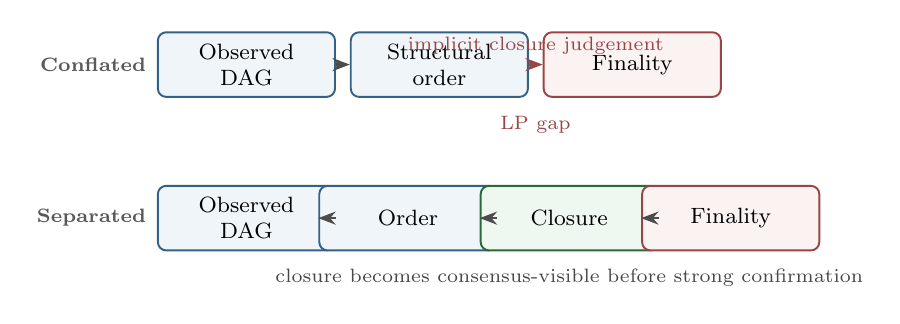
\begin{tikzpicture}[
    stage/.style={draw, rounded corners=3pt, minimum width=2.25cm,
                  minimum height=0.82cm, align=center, font=\footnotesize,
                  line width=0.7pt, fill=white},
    ord/.style={stage, draw=blueblock!75!black, fill=blueblock!8},
    cls/.style={stage, draw=closurecolor!70!black, fill=closurecolor!8},
    fin/.style={stage, draw=redblock!75!black, fill=redblock!8},
    arr/.style={-{Stealth[length=2.2mm]}, line width=0.9pt, draw=black!70},
    warn/.style={-{Stealth[length=2.2mm]}, line width=0.9pt,
                 draw=redblock!75!black, dashed},
    note/.style={font=\scriptsize, align=center, text=black!72},
    group/.style={font=\scriptsize\bfseries, text=black!65}
]
\node[group, anchor=east] at (-0.2,0.95) {Conflated};
\node[ord] (gobs) at (0.95,0.95) {Observed\\DAG};
\node[ord] (gord) at (3.4,0.95) {Structural\\order};
\node[fin] (gfin) at (5.85,0.95) {Finality};
\draw[arr] (gobs) -- (gord);
\draw[warn] (gord) -- node[above, font=\scriptsize, text=redblock!75!black]
    {implicit closure judgement} (gfin);
\node[note, text=redblock!75!black] at (4.62,0.18) {LP gap};

\node[group, anchor=east] at (-0.2,-1.0) {Separated};
\node[ord] (pobs) at (0.95,-1.0) {Observed\\DAG};
\node[ord] (pord) at (3.0,-1.0) {Order};
\node[cls] (pcls) at (5.05,-1.0) {Closure};
\node[fin] (pfin) at (7.1,-1.0) {Finality};
\draw[arr] (pobs) -- (pord);
\draw[arr] (pord) -- (pcls);
\draw[arr] (pcls) -- (pfin);
\node[note] at (5.05,-1.76) {closure becomes consensus-visible before strong confirmation};
\end{tikzpicture}
\caption{Why an explicit closure layer is needed.  Under LP attack, structural
ordering can progress before the dependency world is mature enough for strong
confirmation.  PHASMDAG inserts closure as an explicit protocol stage rather
than leaving that judgement to implementation heuristics.}
\label{fig:semantic_gap}
\end{figure}

\subsection{Formal Problem Definition}

\begin{definition}[The PHASMDAG Problem]\label{def:problem}
Design a DAG consensus protocol that:
\begin{enumerate}[nosep]
    \item preserves GhostDAG's ability to capture structural concurrency,
    \item makes closure maturity a first-class protocol state,
    \item derives finality from both order strength and closure maturity,
    \item maintains security guarantees under the CBM without relying on the
    Decoupling Assumption, and
    \item degrades gracefully under LP attacks and bandwidth congestion.
\end{enumerate}
\end{definition}

% =====================================================================
\section{Protocol Design}\label{sec:design}

\subsection{Three Semantic Layers}

PHASMDAG reasons over three explicit semantic layers:

\begin{description}[nosep]
    \item[Layer A --- Order Layer] determines structural support and preferred
    ordering relations in the DAG.  In PHASMDAG-$v_0$, this layer is fixed to a
    GhostDAG-style \emph{blue-work lineage}; alternative order cores are future
    variants, not part of the base protocol.

    \item[Layer B --- Closure Layer] measures whether a block and its dependency
    world are sufficiently mature, stable, and coherently visible across honest
    nodes.  This is the additional layer absent from GhostDAG-family protocols.

    \item[Layer C --- Finality Layer] derives confirmation/finality from both
    order and closure, rather than from order alone.
\end{description}

The relationship between layers is illustrated in \Cref{fig:layers}.

\begin{figure}[t]
\centering
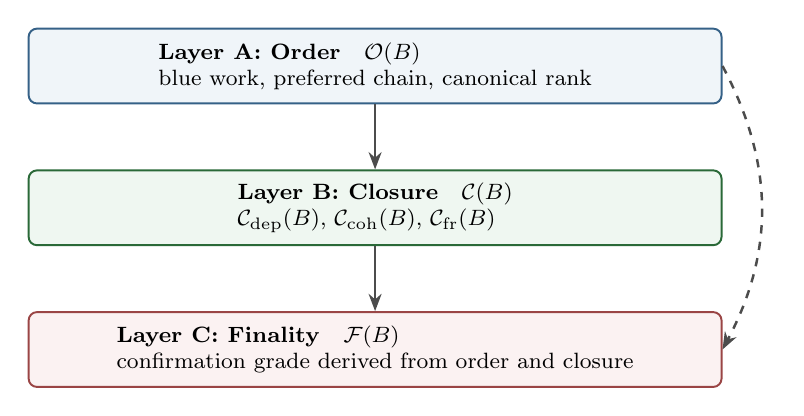
\begin{tikzpicture}[
    layer/.style={draw, rounded corners=3pt, minimum width=8.8cm,
                  minimum height=0.95cm, font=\footnotesize, align=left,
                  line width=0.7pt, inner xsep=7pt, fill=white},
    ord/.style={layer, draw=blueblock!75!black, fill=blueblock!8},
    cls/.style={layer, draw=closurecolor!70!black, fill=closurecolor!8},
    fin/.style={layer, draw=redblock!75!black, fill=redblock!8},
    arr/.style={-{Stealth[length=2.2mm]}, line width=0.9pt, draw=black!70}
]
\node[ord] (A) at (0,0)
    {\textbf{Layer A: Order}\quad $\Ostr(B)$\\blue work, preferred chain, canonical rank};
\node[cls] (B) at (0,-1.8)
    {\textbf{Layer B: Closure}\quad $\Clvl(B)$\\$\Cdep(B)$, $\Ccoh(B)$, $\Cfr(B)$};
\node[fin] (C) at (0,-3.6)
    {\textbf{Layer C: Finality}\quad $\Ffin(B)$\\confirmation grade derived from order and closure};
\draw[arr] (A) -- (B);
\draw[arr] (B) -- (C);
\draw[arr, dashed, bend left=28] (A.east) to (C.east);
\end{tikzpicture}
\caption{The three semantic layers of PHASMDAG.  The Order layer feeds the
Closure layer; both jointly determine the Finality layer.  The dashed arrow
indicates that Order also feeds Finality directly, not only through Closure.}
\label{fig:layers}
\end{figure}

\subsection{Core Quantities}

For each block $B$ in the observed DAG $\Dag = (V, E)$, two core
quantities.

\begin{definition}[Order Strength]\label{def:order_strength}
For PHASMDAG-$v_0$, the \emph{order strength} of block $B$ is the block's
position on the GhostDAG blue-work lineage:
\begin{equation}\label{eq:order_strength}
\Ostr(B) := \mathrm{BlueWork}(B), \qquad \Ostr(B) \in \Rset_{\ge 0}
\end{equation}
a structural support quantity measuring how strongly the DAG structure supports
placing $B$ in the canonical history.
The canonical order rank $r(B)$ is the deterministic rank induced by this
blue-work order core.
\end{definition}

\begin{definition}[Relevant Support Window]\label{def:support_window}
Let $H \in \mathbb{N}$ be a protocol parameter.
The \emph{relevant support window} of block $B$ is
\begin{equation}\label{eq:support_window}
\mathcal{W}_H(B) :=
\{D \in \mathrm{desc}(B) : 0 < r(D) - r(B) \le H\}.
\end{equation}
All closure metrics in PHASMDAG-$v_0$ are computed over $\mathcal{W}_H(B)$ so
that they are bounded, deterministic, and auditable.
\end{definition}

\begin{definition}[Closure Sub-Metrics]\label{def:closure_submetrics}
Let $W(B)$ denote the PoW work attributed to block $B$.
For each $D \in \mathcal{W}_H(B)$, let $\mathbf{1}_{\mathrm{closed}}(D)=1$ if
all protocol-required predecessor objects of $D$ have been observed and
validated at the evaluating node, and $0$ otherwise.
Let $c^\star(B)$ denote the canonical child of $B$ on the blue-work lineage,
and let $\pi_B(D)$ denote the first child of $B$ on the path from $B$ to $D$.
Let $\mathrm{Front}_H(B)$ be the set of maximal blocks in $\mathcal{W}_H(B)$,
and let $f^\star(B) \in \mathrm{Front}_H(B)$ be the frontier tip that extends
$c^\star(B)$ when such a tip exists.
The sub-metrics are defined by:
\begin{align}
\Cdep(B)
&=
\frac{\sum_{D \in \mathcal{W}_H(B)} W(D)\,\mathbf{1}_{\mathrm{closed}}(D)}
{\sum_{D \in \mathcal{W}_H(B)} W(D)}
\label{eq:cdep} \\
\Ccoh(B)
&=
\frac{\sum_{D \in \mathcal{W}_H(B)} W(D)\,\mathbf{1}[\pi_B(D)=c^\star(B)]}
{\sum_{D \in \mathcal{W}_H(B)} W(D)}
\label{eq:ccoh} \\
\Cfr(B)
&=
\frac{W(f^\star(B))}
{\sum_{F \in \mathrm{Front}_H(B)} W(F)}
\label{eq:cfr}
\end{align}
with the convention that each ratio is $0$ when its denominator is $0$.
\end{definition}

\begin{definition}[Closure Level]\label{def:closure_level}
The \emph{closure level} of block $B$ is the deterministic aggregation of the
three closure sub-metrics:
\begin{equation}\label{eq:closure_level}
\Clvl(B) = g_{v_0}\!\bigl(\Cdep(B),\,\Ccoh(B),\,\Cfr(B)\bigr)
\end{equation}
where PHASMDAG-$v_0$ uses the weighted geometric mean
\begin{equation}\label{eq:closure_level_v0}
g_{v_0}(x,y,z) = x^{\eta_{\mathrm{dep}}}
y^{\eta_{\mathrm{coh}}}
z^{\eta_{\mathrm{fr}}},
\qquad
\eta_{\mathrm{dep}}+\eta_{\mathrm{coh}}+\eta_{\mathrm{fr}}=1.
\end{equation}
This aggregation makes a low value in any one dimension visibly reduce the
overall closure score.
\end{definition}

\begin{remark}\label{rem:closure_vs_delay}
$\Clvl(B)$ is \emph{not} a function of observed propagation delay.
It measures structural properties of the dependency world (completeness,
stability, coherence), not temporal observations.
This is a deliberate design choice: observed delays are node-specific and
vulnerable to topology bias~\cite{wu2024security}, whereas structural
completeness can, in principle, be determined deterministically from the DAG
structure that honest nodes eventually agree on.
\end{remark}

\begin{remark}[Why the decomposition matters]\label{rem:closure_decomp}
The protocol now exposes three attack surfaces instead of hiding them inside
one all-purpose closure scalar:
\Cref{eq:cdep} captures dependency completeness,
\Cref{eq:ccoh} captures descendant-support coherence, and
\Cref{eq:cfr} captures frontier stability.
Each can be analysed, simulated, and attacked separately.
\end{remark}
\Cref{fig:closure_components} shows how these three quantities are read off from
the local descendant structure around a block.

\begin{figure}[t]
\centering
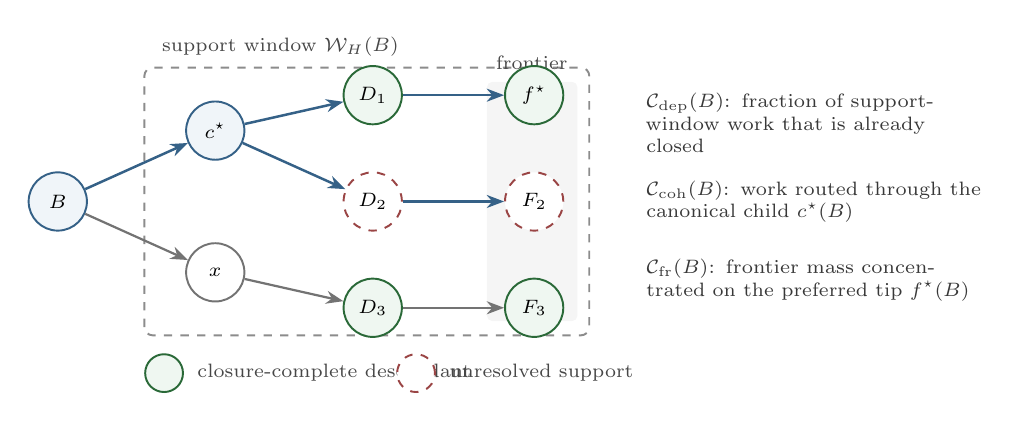
\begin{tikzpicture}[
    x=1cm, y=1cm,
    blk/.style={circle, minimum size=7.4mm, inner sep=0pt, draw=black!55,
                fill=white, line width=0.7pt, font=\scriptsize},
    focus/.style={blk, draw=blueblock!75!black, fill=blueblock!8},
    closed/.style={blk, draw=closurecolor!70!black, fill=closurecolor!8},
    unresolved/.style={blk, draw=redblock!75!black, fill=white, dashed},
    edge/.style={-{Stealth[length=2.2mm]}, line width=0.8pt, draw=black!55},
    pref/.style={-{Stealth[length=2.2mm]}, line width=0.9pt, draw=blueblock!75!black},
    boxlabel/.style={font=\scriptsize, align=left, text=black!78},
    key/.style={font=\scriptsize, text=black!72}
]
\draw[rounded corners=3pt, dashed, draw=black!45, line width=0.7pt]
    (1.1,-1.7) rectangle (6.75,1.7);
\fill[black!4, rounded corners=2pt] (5.45,-1.52) rectangle (6.6,1.52);
\node[key, anchor=south west] at (1.2,1.72) {support window $\mathcal{W}_H(B)$};
\node[key, anchor=south] at (6.02,1.55) {frontier};

\node[focus] (B) at (0,0) {$B$};
\node[focus] (c) at (2,0.9) {$c^\star$};
\node[blk]   (x) at (2,-0.9) {$x$};
\node[closed]     (d1) at (4,1.35) {$D_1$};
\node[unresolved] (d2) at (4,0.0) {$D_2$};
\node[closed]     (d3) at (4,-1.35) {$D_3$};
\node[closed]     (f1) at (6.05,1.35) {$f^\star$};
\node[unresolved] (f2) at (6.05,0.0) {$F_2$};
\node[closed]     (f3) at (6.05,-1.35) {$F_3$};

\draw[pref] (B) -- (c);
\draw[edge] (B) -- (x);
\draw[pref] (c) -- (d1);
\draw[pref] (c) -- (d2);
\draw[edge] (x) -- (d3);
\draw[pref] (d1) -- (f1);
\draw[pref] (d2) -- (f2);
\draw[edge] (d3) -- (f3);

\node[boxlabel, text width=4.25cm, anchor=west] at (7.35,1.0)
    {$\Cdep(B)$: fraction of support-window work that is already closed};
\node[boxlabel, text width=4.25cm, anchor=west] at (7.35,0.0)
    {$\Ccoh(B)$: work routed through the canonical child $c^\star(B)$};
\node[boxlabel, text width=4.25cm, anchor=west] at (7.35,-1.0)
    {$\Cfr(B)$: frontier mass concentrated on the preferred tip $f^\star(B)$};

\node[closed, minimum size=4.8mm] at (1.35,-2.18) {};
\node[key, anchor=west] at (1.65,-2.18) {closure-complete descendant};
\node[unresolved, minimum size=4.8mm] at (4.55,-2.18) {};
\node[key, anchor=west] at (4.85,-2.18) {unresolved support};
\end{tikzpicture}
\caption{Closure decomposition around block $B$.  The support window
$\mathcal{W}_H(B)$ supplies the auditable evidence set; $\Cdep(B)$ measures how
much of that work is closure-complete, $\Ccoh(B)$ measures how much support
flows through the canonical child $c^\star(B)$, and $\Cfr(B)$ measures whether
frontier work is concentrated on the preferred tip $f^\star(B)$.}
\label{fig:closure_components}
\end{figure}

\subsection{Bi-Objective Consensus Functional}

The principal departure in PHASMDAG is the replacement of the purely
structural objective~\eqref{eq:ghostdag_objective} with a bi-objective
functional:

\begin{definition}[Bi-Objective Consensus Functional]\label{def:biobjective}
Given a candidate consensus-supporting structure $S$, the protocol evaluates:
\begin{equation}\label{eq:biobjective}
\Phifn(S) = \Uord(S) - \lambda \cdot \Rcls(S)
\end{equation}
where:
\begin{itemize}[nosep]
    \item $\Uord(S)$ rewards coherent structural order, useful concurrency,
    descendant-backed support, and stable preferred-chain evolution under the
    blue-work order core.
    \item $\Rcls(S)$ is a protocol-visible closure-risk functional rather than a
    prose penalty.
    \item $\lambda > 0$ is a control parameter setting the tradeoff between
    structural concurrency capture and closure conservatism.
\end{itemize}
\end{definition}

\begin{definition}[Closure-Risk Functional]\label{def:rclosure}
For a candidate set $S$, define
\begin{equation}\label{eq:rclosure}
\Rcls(S) =
a\sum_{B\in S}(1-\Cdep(B))
{}+ b\sum_{B\in S}(1-\Ccoh(B))
{}+ c\sum_{B\in S}(1-\Cfr(B))
{}+ d\cdot \Frag(S)
\end{equation}
where $a,b,c,d \ge 0$ are protocol parameters.
The first three terms are block-local penalties.
The last term captures set-level brittleness:
let
\begin{equation}\label{eq:unresolved_set}
\mathcal{U}(B) :=
\{D \in \mathcal{W}_H(B) : \mathbf{1}_{\mathrm{closed}}(D)=0\},
\end{equation}
then
\begin{equation}\label{eq:fragility_coupling}
\Frag(S)
:=
\frac{1}{|P_2(S)|}
\sum_{\{B_i,B_j\}\in P_2(S)}
\frac{\sum_{D \in \mathcal{U}(B_i)\cap \mathcal{U}(B_j)} W(D)}
{\sum_{D \in \mathcal{U}(B_i)\cup \mathcal{U}(B_j)} W(D)},
\end{equation}
with value $0$ when the denominator is $0$.
Here $P_2(S)$ is the set of unordered pairs in $S$.
\end{definition}

\begin{remark}[Auditability of $\Rcls$]\label{rem:rclosure_audit}
\Cref{eq:rclosure} makes closure risk auditable at two levels:
nodes can explain which block-local term depressed a given block's score, and
they can separately inspect whether a set of otherwise acceptable blocks shares
the same unresolved support pockets through $\Frag(S)$.
\end{remark}

This marks the fundamental departure from GhostDAG:
\textbf{the protocol no longer maximises structure alone.}
It instead maximises a combination of structural utility and closure
robustness.

\begin{remark}[$\lambda$ semantics]\label{rem:lambda}
The parameter $\lambda$ has operational and economic semantics:
\begin{itemize}[nosep]
    \item Small $\lambda$: the protocol is more optimistic, capturing more raw
    concurrency but tolerating more closure fragility.
    \item Large $\lambda$: the protocol is more conservative, sacrificing some
    concurrency for stronger closure guarantees.
    \item $\lambda \to 0$: PHASMDAG reduces to GhostDAG (pure structural
    optimisation).
\end{itemize}
Whether $\lambda$ is a static protocol constant or an epoch-level
consensus-updated parameter is an open design choice discussed in
\Cref{sec:open}.
\end{remark}

\subsection{Finality Functional}

\begin{definition}[Closure-Aware Finality]\label{def:finality}
The finality of block $B$ is determined by a joint function:
\begin{equation}\label{eq:finality}
\Ffin(B) = f\bigl(\Ostr(B),\, \Clvl(B),\, D(B)\bigr)
\end{equation}
where $D(B)$ represents settlement depth / descendant accumulation.
A simple parameterised form is:
\begin{equation}\label{eq:finality_simple}
\Ffin(B) = \sigma\bigl(\alpha \cdot \Ostr(B) + \beta \cdot \Clvl(B)
+ \gamma \cdot D(B) - \tau\bigr)
\end{equation}
where $\sigma$ is a monotone squashing or thresholding function, and
$\alpha, \beta, \gamma, \tau$ are protocol parameters.
\end{definition}

This means finality is no longer a direct byproduct of blue-work accumulation.
A block with high order strength but low closure maturity receives only
tentative confirmation; strong confirmation requires both conditions.

\subsection{Three Confirmation Grades}

The protocol exposes three grades of confirmation:

\begin{description}[nosep]
    \item[Grade 1 --- Tentative Ordering]
    Block $B$ is structurally well-placed in the DAG, but closure maturity is
    not yet sufficient for strong trust.
    Formally: $\Ostr(B)$ exceeds a threshold, but $\Clvl(B)$ is below the
    strong-confirmation threshold.

    \item[Grade 2 --- Strong Confirmation]
    Block $B$ has both high structural support and sufficiently high closure
    maturity.
    Formally: both $\Ostr(B)$ and $\Clvl(B)$ exceed their respective
    thresholds.

    \item[Grade 3 --- Deep Settlement]
    Block $B$ has accumulated enough joint support that rollback becomes
    economically or combinatorially negligible.
    Formally: $\Ffin(B)$ exceeds a high-confidence threshold.
\end{description}

This replaces the traditional ``one confirmation number fits all'' model with
semantically differentiated confirmation objects.
The geometry of these grades is illustrated in \Cref{fig:grades_plane}.

\begin{figure}[t]
\centering
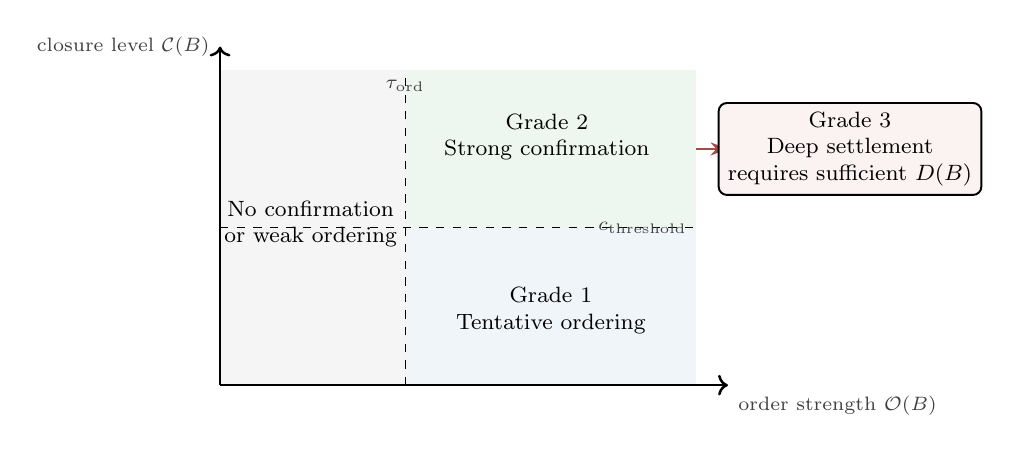
\begin{tikzpicture}[
    x=1cm, y=1cm,
    regionlabel/.style={font=\footnotesize, align=center},
    axislabel/.style={font=\scriptsize, text=black!75},
    callout/.style={draw, rounded corners=3pt, fill=redblock!8,
                    line width=0.7pt, align=center, font=\footnotesize}
]
\fill[black!4] (0,0) rectangle (2.35,4.0);
\fill[blueblock!8] (2.35,0) rectangle (6.05,2.0);
\fill[closurecolor!9] (2.35,2.0) rectangle (6.05,4.0);

\draw[->, line width=0.9pt] (0,0) -- (6.45,0)
    node[below right, axislabel] {order strength $\Ostr(B)$};
\draw[->, line width=0.9pt] (0,0) -- (0,4.3)
    node[left, axislabel] {closure level $\Clvl(B)$};
\draw[dashed] (2.35,0) -- (2.35,4.0) node[below, axislabel] {$\tau_{\mathrm{ord}}$};
\draw[dashed] (0,2.0) -- (6.05,2.0) node[left, axislabel] {$c_{\mathrm{threshold}}$};

\node[regionlabel] at (1.15,2.05) {No confirmation\\or weak ordering};
\node[regionlabel] at (4.2,0.95) {Grade 1\\Tentative ordering};
\node[regionlabel] at (4.15,3.15) {Grade 2\\Strong confirmation};

\draw[-{Stealth[length=2.2mm]}, line width=0.9pt, draw=redblock!80!black]
    (6.05,3.0) -- (6.45,3.0);
\node[callout, minimum width=2.75cm, minimum height=1.1cm] at (8.0,3.0)
    {Grade 3\\Deep settlement\\requires sufficient $D(B)$};
\end{tikzpicture}
\caption{Confirmation-grade geometry.  Grade~1 requires sufficiently strong
structural ordering, Grade~2 additionally requires closure above the strong
confirmation threshold, and Grade~3 adds sufficient settlement depth on top of
Grade~2.}
\label{fig:grades_plane}
\end{figure}

\subsection{Confirmation Invariants}

\begin{invariant}[Tentative Ordering Bounded Churn]\label{inv:tentative}
There exists a protocol parameter $\rho_{\mathrm{tent}}$ such that once a block
$B$ attains Grade~1, any later honest view that still places $B$ in the
canonical order may change its rank by at most $\rho_{\mathrm{tent}}$.
Tentative ordering may move, but only within a bounded local reorder depth.
\end{invariant}

\begin{invariant}[Strong Confirmation Agreement]\label{inv:strong}
No two honest nodes may assign Grade~2 to conflicting blocks at the same
virtual position in the canonical order.
Strong confirmation is therefore a protocol object, not merely a UI label.
\end{invariant}

\begin{invariant}[Deep Settlement Tail]\label{inv:settlement}
There exists a protocol target $\varepsilon_{\mathrm{settle}}$ such that any
block assigned Grade~3 has rollback probability at most
$\varepsilon_{\mathrm{settle}}$ under the stated network and adversarial
assumptions.
\end{invariant}

% =====================================================================
\section{Security Analysis under CBM}\label{sec:security}

\subsection{Threat Model}

The CBM threat model of~\cite{wu2024security} is adopted with three layers:

\begin{enumerate}[nosep]
    \item \textbf{Analytical layer}: an abstract CBM attacker who can partition
    honest nodes into $s$ groups and selectively delay block delivery.
    \item \textbf{Realisable layer}: attacks implementable via BGP hijacking,
    Eclipse attacks, or strategic peer selection.
    \item \textbf{Implementation layer}: representative node behaviour under
    stress, including orphan-pool dynamics and header-body skew.
\end{enumerate}

\subsection{Chain Growth under Closure Awareness}

This subsection is intentionally preliminary.
It does \emph{not} claim a completed security proof for PHASMDAG.
Instead, it records one concrete modelling ansatz for how closure awareness may
change the LP security envelope, assuming the deterministic $v_0$ closure
metric and eventual convergence of its sub-metrics.

\begin{lemma}[Preliminary closure-modulated chain-growth heuristic]\label{lem:closure_growth}
Under CBM with LP attack parameter $s$, let $\Clvl_{\min}(t)$ denote the
minimum closure level among blocks that contribute to the honest chain's
structural support at time $t$.
Under the heuristic assumption that unresolved closure mass linearly modulates
delay exposure, the effective chain growth rate is:
\begin{equation}\label{eq:closure_growth}
g_{\mathrm{PHASM}} = (1 - \sigma)\,\gamma_{\mathrm{eff}}\,f
\end{equation}
where:
\begin{equation}\label{eq:gamma_eff}
\gamma_{\mathrm{eff}}
= \frac{\alpha \cdot \Clvl_{\min}}{1 + \alpha f \cdot
\mathbb{E}[\Delta] \cdot (1 - \Clvl_{\min})}
\end{equation}
\end{lemma}

\begin{proof}[Proof sketch]
Under GhostDAG (\Cref{thm:cbm}), the chain growth rate is
$g = (1-\sigma)\gamma f$ where $\gamma = \alpha/(1 + \alpha f \mathbb{E}[\Delta])$.
The key quantity is $\mathbb{E}[\Delta]$, the expected actual delay including
processing delay from late predecessors.

In PHASMDAG, the bi-objective functional $\Phifn = \Uord - \lambda \Rcls$
weights each block's contribution to structural support by its closure
maturity.  Specifically, a block $B$ with closure level $\Clvl(B)$ contributes
an effective weight of $w(B) = \Clvl(B)$ to the order utility; the remaining
fraction $(1 - \Clvl(B))$ is absorbed by the closure risk penalty.

This means that only the \emph{resolved} portion of the dependency world
contributes to effective chain growth.  The unresolved fraction
$(1 - \Clvl_{\min})$ carries the delay risk.  Substituting
$\mathbb{E}[\Delta] \cdot (1 - \Clvl_{\min})$ for $\mathbb{E}[\Delta]$
in \Cref{thm:cbm}, and noting that the numerator's honest hash power is
modulated by $\Clvl_{\min}$ (since only closure-mature blocks contribute
full weight), we obtain:
\begin{equation*}
\gamma_{\mathrm{eff}} = \frac{\alpha \cdot \Clvl_{\min}}
{1 + \alpha f \cdot \mathbb{E}[\Delta] \cdot (1 - \Clvl_{\min})}
\end{equation*}
When $\Clvl_{\min} = 1$ (full closure), this reduces to $\gamma_{\mathrm{eff}}
= \alpha / (1 + 0) = \alpha$, which is the GhostDAG rate under UDBM with
zero LP effect---consistent with the intuition that full closure maturity
eliminates delay exposure.  When $\Clvl_{\min} = 0$ (complete closure
failure), $\gamma_{\mathrm{eff}} = 0$, reflecting that no effective chain
growth is possible when no block's dependency world is mature.
This derivation should be read as a candidate parameterisation, not as a
finished reduction from the CBM theorem of Wu et al.
\end{proof}

\begin{proposition}[Preliminary dominance region]\label{prop:graceful}
Under LP attack, PHASMDAG's effective security threshold
$\gamma_{\mathrm{eff}}$ dominates GhostDAG's $\gamma$ within the parameter
region
\begin{equation}\label{eq:graceful}
\Clvl_{\min} \ge \frac{1}{1 + 2\alpha f \mathbb{E}[\Delta]}.
\end{equation}
Within this region, the heuristic ansatz of \Cref{lem:closure_growth} implies
$\gamma_{\mathrm{eff}} \ge \gamma$.
\end{proposition}

\begin{proof}[Proof sketch]
Compare $\gamma$ from \Cref{thm:cbm} with $\gamma_{\mathrm{eff}}$ from
\Cref{lem:closure_growth}:
\begin{align}
\gamma &= \frac{\alpha}{1 + \alpha f \cdot \mathbb{E}[\Delta]}
\label{eq:gamma_ghost} \\
\gamma_{\mathrm{eff}} &= \frac{\alpha \cdot \Clvl_{\min}}
{1 + \alpha f \cdot \mathbb{E}[\Delta] \cdot (1 - \Clvl_{\min})}
\label{eq:gamma_closure_modulated}
\end{align}
Cross-multiplying the claim $\gamma_{\mathrm{eff}} \ge \gamma$ gives
\begin{equation*}
\alpha \cdot \Clvl_{\min} \cdot (1 + \alpha f \mathbb{E}[\Delta])
\ge \alpha \cdot (1 + \alpha f \mathbb{E}[\Delta](1 - \Clvl_{\min}))
\end{equation*}
Simplify (both sides have $\alpha > 0$):
\begin{equation*}
\Clvl_{\min} + \alpha f \mathbb{E}[\Delta] \cdot \Clvl_{\min}
\ge 1 + \alpha f \mathbb{E}[\Delta] - \alpha f \mathbb{E}[\Delta] \cdot \Clvl_{\min}
\end{equation*}
Rearranging:
\begin{equation*}
2 \alpha f \mathbb{E}[\Delta] \cdot \Clvl_{\min} + \Clvl_{\min} - 1
\ge 0
\end{equation*}
This holds when $\Clvl_{\min}$ is sufficiently large relative to the
LP effect.  Specifically, the inequality holds when
$\Clvl_{\min} \ge 1 / (1 + 2\alpha f \mathbb{E}[\Delta])$.
Since the right-hand side is always $< 1$, there exists a non-trivial
region where the heuristic threshold of PHASMDAG exceeds GhostDAG's.
\end{proof}

\begin{remark}[Interpretation cost of closure awareness]\label{rem:closure_cost}
\Cref{prop:graceful} does \emph{not} establish a universal improvement result.
It identifies a preliminary dominance region under the specific heuristic
ansatz of \Cref{lem:closure_growth}.
The cost is that blocks with $\Clvl < 1$ receive weaker finality
(\Cref{def:finality}), which means the protocol may delay strong confirmation
for blocks whose dependency world is immature.
This behaviour is methodologically preferable: strong confirmation should be
delayed rather than granted on the basis of a structural score that ignores
closure fragility.
\end{remark}

\subsection{Comparison with GhostDAG under LP Attack}

\begin{table}[t]
\centering
\caption{Preliminary security behaviour comparison under LP attack}
\label{tab:comparison}
\small
\renewcommand{\arraystretch}{1.1}
\begin{tabularx}{0.96\textwidth}{@{}L{3.2cm}YY@{}}
\toprule
\textbf{Property} & \textbf{GhostDAG} & \textbf{PHASMDAG} \\
\midrule
Chain growth rate
    & $g = (1{-}\sigma)\gamma f$
    & $g = (1{-}\sigma)\gamma_{\mathrm{eff}} f$ \\
Security threshold
    & $\beta < \gamma$
    & candidate $\beta < \gamma_{\mathrm{eff}}$ \\
Delay exposure
    & $\mathbb{E}[\Delta]$ (unmodulated)
    & $\mathbb{E}[\Delta]\cdot(1{-}\Clvl_{\min})$ \\
Closure fragility
    & Invisible to protocol
    & First-class state $\Clvl(B)$ \\
Strong finality basis
    & $\Ostr(B)$ alone
    & $\Ostr(B) \wedge \Clvl(B)$ \\
\bottomrule
\end{tabularx}
\end{table}

\Cref{tab:comparison} summarises the key differences.
The essential observation is that PHASMDAG \emph{absorbs} the LP effect into
the protocol's mathematical core rather than treating it as an external
implementation concern.

\subsection{Quality under Heterogeneous Visibility}

Under LP attack, different honest nodes may have different views of the DAG.
GhostDAG's security proofs assume that honest nodes converge to consistent
blue-work orderings; under CBM, this convergence may be delayed or incomplete.

\begin{conjecture}[Closure coherence theorem target]\label{conj:coherence}
Under CBM with honest majority, if $\Clvl(B) \ge c_{\mathrm{threshold}}$ at
some honest node $v$, then within bounded additional time $\Delta_{\mathrm{coherence}}$,
all honest nodes will also observe $\Clvl(B) \ge c_{\mathrm{threshold}} - \epsilon$
for some small $\epsilon > 0$.
\end{conjecture}

\noindent This conjecture, if proven, would establish that closure level
converges across honest nodes---a prerequisite for closure-aware finality to be
consistent.  It is the \emph{central theorem target} of PHASMDAG:
without sufficient convergence of $\Cdep$, $\Ccoh$, and $\Cfr$, Grade~2 cannot
be a consensus-meaningful object.
Its proof or disproof is therefore a primary goal of the formal modelling
roadmap (\Cref{sec:formal}).

\subsection{Incentive Compatibility and Closure Manipulation}\label{sec:incentive}

Introducing $\Clvl(B)$ and $\Rcls(S)$ as first-class protocol objects creates
a new strategic attack surface that does not exist in GhostDAG.  In GhostDAG,
the only rational miner behaviour is to extend the heaviest blue-work chain;
there is no protocol-internal incentive to manipulate structural scores.
In PHASMDAG, miners may profit from manipulating closure evidence.
This draft therefore does \emph{not} claim that honest, immediate broadcasting
is already a Nash equilibrium under PHASMDAG.

\paragraph{Closure suppression.}
A miner could withhold a predecessor block $B^*$ to deliberately depress
$\Clvl(B)$ for a rival's blocks that reference $B^*$ transitively.
This delays the rival's strong confirmation and may shift the preferred-chain
tip toward the attacker's own blocks, since $\Rcls$ penalises the rival's
dependency fragility.

\paragraph{Closure inflation.}
Conversely, a miner could strategically release closure evidence (by
broadcasting withheld predecessors) at a time chosen to maximise the boost to
their own blocks' $\Clvl$, potentially timing the release to outcompete a
rival's chain tip just before a difficulty retarget.

\paragraph{Frontier manipulation.}
Since $\Clvl(B)$ depends on descendant support and frontier concentration
(\Cref{eq:ccoh,eq:cfr}),
a miner could mine descendant blocks that strategically include or exclude
closure-confirming references, steering the frontier to inflate or suppress
$\Clvl$ for selected blocks.

These threats are not theoretical curiosities---they are the direct
consequence of making closure a consensus-relevant quantity.
The full game-theoretic treatment is left for future work, but the
present paper identifies the
following as \emph{required incentive-compatibility goals} for any viable
PHASMDAG specification:
\begin{enumerate}[nosep]
    \item \textbf{Non-profitability of suppression}: withholding predecessors
    should not yield a net revenue advantage, accounting for the attacker's
    own lost block rewards and the cost of maintaining the suppression.
    \item \textbf{Convergence under strategic release}: even if miners
    strategically time the release of closure evidence, $\Clvl(B)$ should
    converge to the same value it would have reached under honest immediate
    broadcasting, within bounded additional time.
    \item \textbf{Sybil resistance}: cheap creation of low-work descendant
    blocks must not inflate $\Clvl(B)$; the work-weighted definitions in
    \Cref{eq:cdep,eq:ccoh,eq:cfr} are intended to enforce this.
\end{enumerate}

\begin{remark}[Relationship to selfish mining]\label{rem:selfish}
Closure manipulation is structurally similar to selfish mining~\cite{zhang2019common}:
both exploit information asymmetry and timing control.
However, closure manipulation operates on a different axis---it manipulates
\emph{dependency maturity} rather than \emph{structural weight}---and may
interact non-trivially with selfish mining strategies.
A complete analysis of the joint strategy space is an important direction for
future work.
\end{remark}

% =====================================================================
\section{Formal Modelling Approach}\label{sec:formal}

This section develops a compositional formal model aligned with the three
semantic layers.

\subsection{Compositional State Machine}

Each block $B$ maintains three logical state components:

\begin{enumerate}[nosep]
    \item \textbf{Structural state} $\Sigma_{\mathrm{ord}}(B)$:
    parent set, selected-parent relation, blue-work score, ordering rank.
    This is essentially the existing GhostDAG state.

    \item \textbf{Closure state} $\Sigma_{\mathrm{cls}}(B)$:
    relevant support window $\mathcal{W}_H(B)$, the three sub-metrics
    $\Cdep(B)$, $\Ccoh(B)$, $\Cfr(B)$, unresolved-support set
    $\mathcal{U}(B)$, and aggregate closure level $\Clvl(B)$.

    \item \textbf{Finality state} $\Sigma_{\mathrm{fin}}(B)$:
    tentative inclusion status, strong confirmation status, settlement
    confidence $\Ffin(B)$.
\end{enumerate}

The full state machine is the product
$\Sigma(B) = \Sigma_{\mathrm{ord}}(B) \times
\Sigma_{\mathrm{cls}}(B) \times \Sigma_{\mathrm{fin}}(B)$,
with admissible transitions defined by the protocol rules.
The transition order is strict: $\Sigma_{\mathrm{ord}}$ is computed first
(since closure depends on structural state), then $\Sigma_{\mathrm{cls}}$,
then $\Sigma_{\mathrm{fin}}$.

\subsection{Local Views and Disagreement Metrics}

The key modelling difficulty is that PHASMDAG is evaluated under partial and
heterogeneous visibility.
The protocol therefore requires an explicit notation for node-local views and
for cross-node disagreement in closure scores.

\begin{definition}[Node-Local DAG View]\label{def:local_view}
Let $\Dag_v(t)$ denote the accepted header-DAG observed by honest node $v$ at
time $t$.
All protocol quantities are node-local during execution:
\[
\Ostr_v(B,t), \qquad \Clvl_v(B,t), \qquad \Ffin_v(B,t), \qquad
\Phifn_v(S,t).
\]
Consensus safety requires that these local quantities converge sufficiently
fast after network stabilisation.
\end{definition}

\begin{definition}[Closure Disagreement]\label{def:closure_gap}
For any block $B$ visible to the honest node set $H_t$ at time $t$, define the
honest-node closure disagreement by
\begin{equation}\label{eq:closure_gap}
\Delta_{\Clvl}(B,t)
:=
\max_{u,v \in H_t}
\left|\Clvl_u(B,t) - \Clvl_v(B,t)\right|.
\end{equation}
The central modelling objective is to show that $\Delta_{\Clvl}(B,t)$ becomes
small quickly enough to support consistent Grade~2 decisions.
\end{definition}

\begin{definition}[Closure-Coherent Strong Confirmation Target]\label{def:coherent_strong}
A block $B$ is said to satisfy the \emph{closure-coherent strong-confirmation
target} at time $t$ if
\begin{equation}\label{eq:coherent_strong}
\min_{v \in H_t} \Clvl_v(B,t) \ge c_{\mathrm{threshold}}
\qquad\text{and}\qquad
\Delta_{\Clvl}(B,t) \le \varepsilon_{\mathrm{coh}}
\end{equation}
for a protocol tolerance $\varepsilon_{\mathrm{coh}} > 0$.
\Cref{conj:coherence} may then be read as a theorem target asserting eventual
attainment of~\eqref{eq:coherent_strong} for structurally supported honest
blocks.
\end{definition}
This convergence target is visualised in \Cref{fig:closure_convergence}.

\begin{figure}[t]
\centering
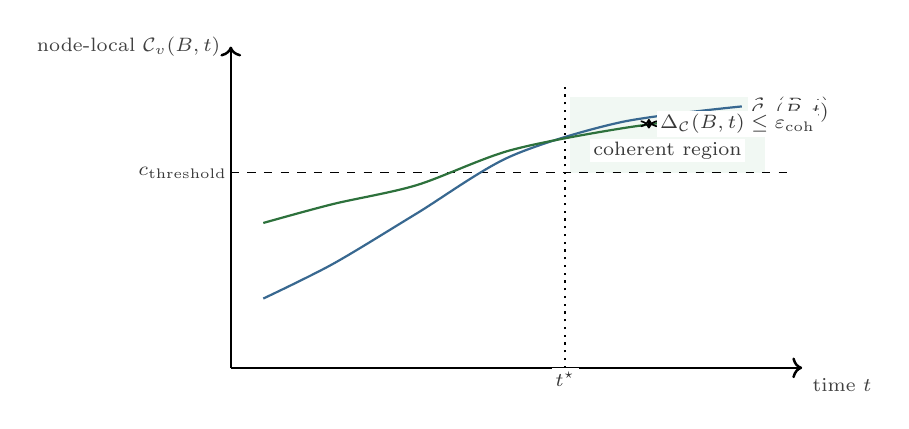
\begin{tikzpicture}[
    x=1.18cm, y=4.0cm,
    axislabel/.style={font=\scriptsize, text=black!75},
    lab/.style={font=\scriptsize, fill=white, inner sep=1.2pt, text=black!78}
]
\fill[closurecolor!7] (3.65,0.62) rectangle (5.75,0.86);
\draw[->, line width=0.9pt] (0,0) -- (6.15,0)
    node[below right, axislabel] {time $t$};
\draw[->, line width=0.9pt] (0,0) -- (0,1.02)
    node[left, axislabel] {node-local $\Clvl_v(B,t)$};
\draw[dashed] (0,0.62) -- (6.0,0.62);
\node[lab, anchor=east] at (0,0.62) {$c_{\mathrm{threshold}}$};

\draw[blueblock!80!black, thick]
    plot[smooth] coordinates {(0.35,0.22) (1.1,0.33) (2.0,0.49) (3.0,0.67) (4.2,0.78) (5.5,0.83)};
\draw[closurecolor!75!black, thick]
    plot[smooth] coordinates {(0.35,0.46) (1.1,0.52) (2.0,0.58) (3.0,0.69) (4.2,0.76) (5.5,0.81)};

\node[lab, anchor=west] at (5.56,0.83) {$\Clvl_u(B,t)$};
\node[lab, anchor=west] at (5.56,0.81) {$\Clvl_v(B,t)$};
\draw[dotted, thick] (3.6,0) -- (3.6,0.9);
\node[lab, anchor=north] at (3.6,0) {$t^\star$};
\draw[<->, semithick] (4.5,0.76) -- (4.5,0.79);
\node[lab, anchor=west] at (4.58,0.775) {$\Delta_{\Clvl}(B,t) \le \varepsilon_{\mathrm{coh}}$};
\node[lab] at (4.7,0.69) {coherent region};
\end{tikzpicture}
\caption{Closure coherence as a convergence target.  Strong confirmation should
only become globally meaningful once node-local closure estimates are both
above $c_{\mathrm{threshold}}$ and sufficiently close to one another.}
\label{fig:closure_convergence}
\end{figure}

\subsection{Block Processing Algorithm}

\Cref{alg:process} specifies the high-level block processing pipeline for
PHASMDAG, making the three-layer computation order explicit.

\begin{algorithm}[t]
\caption{PHASMDAG Block Processing}\label{alg:process}
\begin{algorithmic}[1]
\Require Incoming block $B_{\mathrm{new}}$ with parent set $P$
\Ensure Updated DAG state $\Sigma$
\Statex
\State \textbf{// --- Layer A: Order ---}
\State Validate header in isolation (PoW, timestamp, format) \Comment{Same as GhostDAG}
\State Check all parents exist in $\Sigma_{\mathrm{ord}}$ \Comment{\texttt{check\_parents\_exist}}
\State Compute $\Ostr(B_{\mathrm{new}})$ and $r(B_{\mathrm{new}})$ via blue-work ordering
\State Select preferred parent, compute mergeset, colour blue/red
\State Update $\Sigma_{\mathrm{ord}}(B_{\mathrm{new}})$
\Statex
\State \textbf{// --- Layer B: Closure ---}
\State Identify affected ancestors $A$ whose support windows include $B_{\mathrm{new}}$
\For{each affected block $A$}
    \State Update $\mathcal{W}_H(A)$ and $\mathcal{U}(A)$
    \State Recompute $\Cdep(A)$, $\Ccoh(A)$, and $\Cfr(A)$ \Comment{Approach A / $v_0$}
    \State $\Clvl(A) \gets g_{v_0}\!\bigl(\Cdep(A), \Ccoh(A), \Cfr(A)\bigr)$
\EndFor
\State Initialise $\Sigma_{\mathrm{cls}}(B_{\mathrm{new}})$
\Statex
\State \textbf{// --- Layer C: Finality ---}
\State Compute $\Ffin(B) = f(\Ostr(B), \Clvl(B), D(B))$ for affected blocks
\State Assign confirmation grade:
\If{$\Ffin(B) \ge \tau_{\mathrm{settle}}$}
    \State Grade 3: Deep Settlement
\ElsIf{$\Ostr(B) \ge \tau_{\mathrm{ord}} \wedge \Clvl(B) \ge c_{\mathrm{threshold}}$}
    \State Grade 2: Strong Confirmation
\ElsIf{$\Ostr(B) \ge \tau_{\mathrm{ord}}$}
    \State Grade 1: Tentative Ordering
\Else
    \State No confirmation
\EndIf
\State Update $\Sigma_{\mathrm{fin}}(B_{\mathrm{new}})$ and affected blocks
\Statex
\State \textbf{// --- Propagation decision ---}
\State Compute $\Phifn(S)$ for candidate mining templates
\State Select template maximising $\Uord - \lambda \Rcls$
\end{algorithmic}
\end{algorithm}

\subsection{Closure Level Computation}

The most critical modelling challenge is the computation of $\Clvl(B)$.
PHASMDAG now treats this as a family of explicitly separated design choices,
with one standardised instantiation and one experimental variant.

\paragraph{Approach A: Deterministic attestation-based closure ($v_0$).}
Approach~A is the \textbf{only} standardised closure computation in
PHASMDAG-$v_0$.
Its simplest descendant-attestation form is the PoW-weighted statistic
\begin{equation}\label{eq:closure_attestation_work}
\Clvl_A(B) =
\frac{\sum_{B' \in \mathrm{desc}(B),\;\mathbf{1}_{\mathrm{closed}}(B')=1} W(B')}
{\sum_{B' \in \mathrm{desc}(B)} W(B')}.
\end{equation}
Here $W(B')$ denotes the PoW weight, accumulated work, or
difficulty-equivalent contribution of descendant block $B'$.
This makes closure evidence an economic-security quantity rather than a raw
descendant count, and prevents a minority miner from cheaply inflating
closure with low-value descendants alone.
It instantiates $\Cdep(B)$, $\Ccoh(B)$, and $\Cfr(B)$ exactly as in
\Cref{eq:cdep,eq:ccoh,eq:cfr} and aggregates them with
\Cref{eq:closure_level_v0}.
Equation~\eqref{eq:closure_attestation_work} is the unwindowed intuition;
PHASMDAG-$v_0$ implements the same idea through the bounded support-window
version $\Cdep(B)$ in \Cref{eq:cdep}.
It uses only structural evidence observable in the accepted header-DAG plus the
validation state required for $\mathbf{1}_{\mathrm{closed}}$.
This makes the metric deterministic, decomposable, and auditable.

\paragraph{Approach B: Probabilistic delay-posterior closure.}
Define $\Clvl(B)$ as the probability that $B$'s full dependency world has
been received by a sufficient fraction of honest nodes:
\begin{equation}\label{eq:closure_prob}
\Clvl_B(B) = \Pr\!\Bigl[\text{fraction of honest nodes that have accepted
all preds of } B \ge \theta \;\Big|\; \text{observed evidence}\Bigr]
\end{equation}
This is more expressive---it can incorporate timing evidence and network
models---but harder to compute consistently across nodes and harder to prove
secure.

\begin{table}[t]
\centering
\caption{Closure computation strategies}
\label{tab:closure_approaches}
\begin{tabular}{@{}lcc@{}}
\toprule
\textbf{Property} & \textbf{Approach A} & \textbf{Approach B} \\
\midrule
Deterministic across nodes & Strong & Weak--Medium \\
Responsiveness & Lower & Higher \\
Formal proof friendliness & High & Low \\
Topology bias risk & Low & Higher \\
Implementation complexity & Lower & Higher \\
\bottomrule
\end{tabular}
\end{table}

\begin{remark}[Version policy for closure computation]\label{rem:closure_approaches}
Approach~A is the reference instantiation for PHASMDAG-$v_0$.
Approach~B remains explicitly experimental.
This is a versioning decision, not merely a modelling preference: the base
protocol optimises for determinism and proof-friendliness first.
\end{remark}

\subsection{Parameter Space}

The protocol introduces the following parameters that must be analysed formally:

\begin{table}[tbp]
\centering
\caption{Protocol parameter space}
\label{tab:params}
\small
\renewcommand{\arraystretch}{1.1}
\begin{tabularx}{0.98\textwidth}{@{}L{2.7cm}L{2.6cm}Y@{}}
\toprule
\textbf{Parameter} & \textbf{Type} & \textbf{Constraints} \\
\midrule
$\lambda$ & Protocol-level & $v_0$: static consensus constant; dynamic
adjustment excluded from initial model (\Cref{sec:open}) \\
$H$ & Closure window & Support-horizon size for $\mathcal{W}_H(B)$;
must be large enough to capture relevant descendant evidence \\
$\eta_{\mathrm{dep}}, \eta_{\mathrm{coh}}, \eta_{\mathrm{fr}}$ & Aggregation &
Non-negative and sum to $1$ in \Cref{eq:closure_level_v0} \\
$a,b,c,d$ & Closure-risk weights & Non-negative; determine auditably how
$\Rcls(S)$ trades block-local vs.\ set-level fragility \\
$\alpha, \beta, \gamma, \tau$ & Finality function & Must ensure monotonicity
of $\Ffin$ in both $\Ostr$ and $\Clvl$ \\
$c_{\mathrm{threshold}}$ & Closure & Minimum $\Clvl$ for strong confirmation \\
$\rho_{\mathrm{tent}}$ & Tentative ordering & Maximum permitted rank churn for
Grade~1 (\Cref{inv:tentative}) \\
$\varepsilon_{\mathrm{settle}}$ & Settlement target & Maximum rollback tail for
Grade~3 (\Cref{inv:settlement}) \\
$\Clvl$ definition & Protocol design & $v_0$: Approach~A only; Approach~B is
experimental (\Cref{rem:closure_approaches}) \\
\bottomrule
\end{tabularx}
\end{table}

\subsection{Formal Verification Targets}

The following properties are targets for formal verification:

\begin{enumerate}[nosep]
    \item \textbf{Tentative bounded churn}: prove or bound
    \Cref{inv:tentative} under the blue-work order core.
    \item \textbf{Strong-confirmation safety}: prove
    \Cref{inv:strong}, namely that no two honest nodes assign conflicting
    Grade~2 confirmations at the same virtual position.
    \item \textbf{Settlement tail}: prove or upper-bound
    \Cref{inv:settlement}.
    \item \textbf{Liveness}: every honestly mined block eventually reaches
    tentative ordering (Grade~1) if the network eventually stabilises.
    \item \textbf{Closure coherence}: establish or refute
    \Cref{conj:coherence}, which is the central theorem target of the protocol.
    \item \textbf{Dominance-region validation}: determine whether the heuristic
    region in \Cref{prop:graceful} survives a full CBM proof or only a
    simulation-level approximation.
\end{enumerate}

% =====================================================================
\section{Engineering Verification}\label{sec:verification}

\subsection{Simulation Methodology}

The simulation programme is based on an extension of the
SimBlock~\cite{aoki2019simblock} framework to model
CBM conditions:

\begin{enumerate}[nosep]
    \item \textbf{Network model}: replace the uniform delay model with CBM,
    incorporating bandwidth limits and per-block propagation delays.
    \item \textbf{LP attack simulation}: implement the $s$-group partition
    attack from~\cite{wu2024security}, allowing the attacker to selectively
    delay block delivery to specific node groups.
    \item \textbf{Bandwidth congestion}: simulate Block Jam by enforcing a
    global bandwidth cap and measuring propagation delays as a function of
    utilisation.
    \item \textbf{Closure tracking}: augment each simulated node with the
    $v_0$ closure computation (Approach~A) and track $\Clvl(B)$ over time.
\end{enumerate}

\subsection{Evaluation Metrics}

The evaluation is organised around the following metrics, following the common-metrics
framework of~\cite{zhang2019common}:

\begin{table}[tbp]
\centering
\caption{Evaluation metrics}
\label{tab:metrics}
\small
\renewcommand{\arraystretch}{1.1}
\begin{tabularx}{0.94\textwidth}{@{}L{4.1cm}Y@{}}
\toprule
\textbf{Metric} & \textbf{Description} \\
\midrule
Chain growth rate $g$
    & Blocks per second entering the canonical order \\
Heuristic effective security threshold $\gamma_{\mathrm{eff}}$
    & Candidate minimum honest fraction for security under LP \\
Realised TPS
    & Actual transaction throughput under imperfect networks \\
Tentative confirmation latency
    & Time from block creation to Grade~1 \\
Strong confirmation latency
    & Time from block creation to Grade~2 \\
Deep settlement latency
    & Time from block creation to Grade~3 \\
Closure convergence time
    & Time for $\Clvl(B)$ to reach $c_{\mathrm{threshold}}$ across honest
    nodes \\
P95/P99 finality tail
    & Tail behaviour of confirmation latency under stress \\
\bottomrule
\end{tabularx}
\end{table}

\subsection{Comparative Evaluation Plan}

\begin{enumerate}[nosep]
    \item \textbf{Baseline}: GhostDAG under UDBM (optimistic reference).
    \item \textbf{GhostDAG under CBM}: GhostDAG with LP attack and bandwidth
    congestion, no mitigations.
    \item \textbf{GhostDAG + engineering mitigations}: GhostDAG with
    header-first, dependency-aware relay, and telemetry.
    \item \textbf{PHASMDAG under CBM}: PHASMDAG with $\Clvl$ computation
    (Approach~A) and bi-objective functional, under the same CBM conditions.
\end{enumerate}

The comparison between configurations~(3) and~(4) directly tests
\Cref{prop:engineering_ceiling}: does the protocol-level closure awareness
of PHASMDAG provide security benefits beyond what engineering mitigations
can achieve?

\subsection{Complexity and Incremental Computation}\label{sec:complexity}

The introduction of $\Sigma_{\mathrm{cls}}$ and $\Sigma_{\mathrm{fin}}$
state machines, frontier stability tracking, and closure attestation caches
raises legitimate concerns about computational overhead.  A protocol that is
theoretically sound but practically unrunnable serves no one.
Incremental computation is therefore stipulated as a strict prerequisite for
$v_0$, not an afterthought.

The critical metrics that must be evaluated and bounded before a PHASMDAG
prototype is considered viable are:

\begin{enumerate}[nosep]
    \item \textbf{Amortised per-block update cost for $\Clvl(B)$}:
    Computing $\Clvl(B)$ for a new block requires updating the three
    sub-metrics over the affected support windows.
    Under Approach~A (\Cref{eq:cdep,eq:ccoh,eq:cfr}), this can be formulated
    incrementally: when a new block $B_{\mathrm{new}}$ arrives, only its direct
    work contribution and its canonical-child / frontier relations need to be
    propagated to affected ancestors.
    The target is $O(|\mathrm{parents}|)$ per block, not $O(|\mathrm{ancestors}|)$.

    \item \textbf{Memory footprint of closure-state indices and attestation caches}:
    Each block must store: (a) the cumulative work mass needed for
    $\Cdep(B)$, (b) support-window routing metadata needed for $\Ccoh(B)$, and
    (c) frontier concentration metadata needed for $\Cfr(B)$.
    These are all bounded by the finite support window $H$ and can be encoded as
    compact additive counters plus small frontier indices rather than as a full
    descendant list.

    \item \textbf{Incremental recomputation depth}:
    When $\Clvl(B)$ changes (because a new descendant arrived or a predecessor
    was resolved), closure scores must be updated along the \emph{affected
    descendant frontier}---not the entire DAG.  The expected frontier size is
    bounded by the merge depth and the number of recent blocks, both of which
    are $O(K)$ in the current GhostDAG implementation.

    \item \textbf{Lazy recomputation for deep historical blocks}:
    Blocks deeper than the finality depth can be considered settled; their
    $\Clvl$ values are no longer consensus-relevant and need not be
    recomputed.  Pruning strategies can treat $\Clvl$ computation similarly to
    how existing GhostDAG implementations prune anticone data beyond the
    pruning depth.
\end{enumerate}

\begin{remark}[Computational feasibility of Approach A]\label{rem:approach_a_cost}
Approach~A is specifically designed for incremental computation:
the work-weighted numerators and denominators in
\Cref{eq:cdep,eq:ccoh,eq:cfr} are additive or frontier-local quantities that
can be updated without re-walking the entire descendant cone.
This contrasts with Approach~B (\Cref{eq:closure_prob}), which would require
Bayesian updates over the entire ancestor set and therefore lacks a similarly
clean incremental path.
This is an additional reason to prefer Approach~A for $v_0$.
\end{remark}

\subsection{Phased Verification Roadmap}

\begin{table}[tbp]
\centering
\caption{Phased verification roadmap}
\label{tab:roadmap}
\small
\renewcommand{\arraystretch}{1.1}
\begin{tabularx}{0.98\textwidth}{@{}L{1.2cm}L{1.7cm}Y@{}}
\toprule
\textbf{Phase} & \textbf{Timeline} & \textbf{Deliverables} \\
\midrule
1 & 0--6\,mo
  & Formal model: define $\Ostr$, $\Cdep$, $\Ccoh$, $\Cfr$, $\Clvl$, and $\Ffin$;
    specify state machine and admissible transitions \\
2 & 6--12\,mo
  & Simulation: implement CBM/LP scenarios in SimBlock;
    compare GhostDAG vs PHASMDAG under identical conditions \\
3 & 12--18\,mo
  & Security analysis: chain growth under joint order/closure semantics;
    quality under heterogeneous visibility;
    adversarial threshold as function of closure degradation \\
4 & 18--24\,mo
  & Prototype: implement order layer + closure tracking;
    expose three confirmation grades;
    evaluate on a controlled experimental network \\
\bottomrule
\end{tabularx}
\end{table}

Note that Phases 1--2 can proceed in parallel with the engineering mitigations
(header-first, telemetry, dependency-aware relay) and other implementation-level
studies of GhostDAG.  The CBM-GhostDAG security proof may be read as a decision
gate: if it indicates that engineering mitigations suffice at the target BPS,
PHASMDAG may remain chiefly a research direction; if not, it may warrant
treatment as a more substantial redesign path.

% =====================================================================
\section{Discussion}\label{sec:discussion}

\subsection{Comparison with Delay-Weighted Colouring}

An alternative approach to handling LP effects is delay-weighted
colouring---promoting GhostDAG's binary blue/red colouring to a continuous
weight based on observed propagation delay.
For a consensus-visible $v_0$ design, PHASMDAG's $\Rcls$ is the more
analytically coherent
choice:

\begin{table}[tbp]
\centering
\caption{Delay-weighted colouring vs.\ PHASMDAG $\Rcls$}
\label{tab:dwc_vs_closure_risk}
\small
\renewcommand{\arraystretch}{1.1}
\begin{tabularx}{0.98\textwidth}{@{}L{3.2cm}YY@{}}
\toprule
\textbf{Dimension} & \textbf{Delay-Weighted} & \textbf{PHASMDAG $\Rcls$} \\
\midrule
Penalisation target
    & Observed delay
    & Dependency fragility \\
Topology bias risk
    & High
    & Low \\
Conceptual cleanliness
    & Temporal signal $\to$ consensus weight
    & Structural robustness $\to$ consensus function \\
Node consistency
    & Different nodes see different delays
    & Structural properties converge \\
\bottomrule
\end{tabularx}
\end{table}

The key insight is that $\Rcls$ penalises \emph{structural fragility}
(dependency incompleteness, frontier instability) rather than \emph{temporal
observations} (how long a block took to arrive).
Since structural properties of the DAG eventually converge across honest nodes,
$\Rcls$ is less vulnerable to the topology bias identified
in~\cite{wu2024security,zhang2019common}.

\subsection{Failure Modes and Design Risks}

The proposal is best read alongside an explicit account of its likely failure
modes.  The most important of these are:
\begin{itemize}[nosep]
    \item \textbf{Closure metric too conservative}: $\Cdep$, $\Ccoh$, or
    $\Cfr$ may converge too slowly, causing avoidable TPS and finality
    regressions.
    \item \textbf{Closure metric too weak}: an under-specified sub-metric may
    merely rename the LP attack surface instead of eliminating it.
    \item \textbf{$\lambda$ badly chosen}: too small and the protocol collapses
    back toward GhostDAG-style optimism; too large and it becomes quasi-serial
    and over-conservative.
    \item \textbf{Set-level fragility under-modelled}: if $\Frag(S)$ is too
    weak, individually acceptable blocks may still form a collectively brittle
    support structure.
    \item \textbf{Closure coherence slower than assumed}: if the sub-metrics do
    not converge quickly enough across honest nodes, Grade~2 cannot be treated
    as a safe consensus object.
    \item \textbf{Semantic interface complexity}: the three-grade finality
    model may be theoretically well motivated yet difficult to expose through
    higher-layer interfaces without misinterpretation.
\end{itemize}

\subsection{Open Problems}\label{sec:open}

\paragraph{$\Clvl(B)$ semantics.}
The decomposition of $\Clvl(B)$ is now explicit, but the central open problem
is no longer ``what are the parts?'' but ``do the parts converge enough across
honest nodes?''
Approach~A (\Cref{rem:closure_approaches}) gives deterministic rules for
$\Cdep$, $\Ccoh$, and $\Cfr$, yet the theorem target remains
\Cref{conj:coherence}: proving that these sub-metrics stabilise quickly enough
to support consistent Grade~2 confirmation.
That is the hardest unresolved problem in the paper.

\paragraph{$\lambda$ consensus consistency.}
For $v_0$, $\lambda$ is a \textbf{static protocol constant}, fixed at genesis
or updated only via hard fork.  This is the simplest design that guarantees
consensus consistency: all nodes trivially agree on $\lambda$.

However, the optimal $\lambda$ varies with network conditions: small $\lambda$
is optimal under light load, large $\lambda$ under congestion.  A dynamic
$\lambda$ that adapts to observed network stress---analogous to a
control-theoretic PID controller---is a conceptually interesting but
consensus-sensitive extension.
The risk is total consensus failure if nodes have slightly misaligned
observation windows or if the congestion signal itself is manipulated by an
attacker.

Dynamic $\lambda$ is therefore framed as a \emph{control-theoretic extension
candidate}, excluded from the initial formal model due to:
\begin{enumerate}[nosep]
    \item Consensus-consistency risk: nodes observing different network
    conditions would compute different $\lambda$, leading to divergent chain
    tips.
    \item Signal manipulation vectors: an attacker could manipulate the
    congestion signal (e.g., via bandwidth throttling) to trick honest nodes
    into an unfavourable $\lambda$.
\end{enumerate}
Nodes \emph{could} compute a local, non-consensus advisory metric
$\lambda_{\mathrm{estimate}}$ strictly for simulation, operator dashboards,
and telemetry.  This metric must not bear upon block validity or consensus
state; it is purely informational.
A potential middle ground for future work is epoch-level consensus updates,
similar to difficulty adjustment in Bitcoin, but this requires careful
analysis of the update rule's attack surface.

\paragraph{Fork distance from GhostDAG.}
PHASMDAG should perhaps not be understood as a minor variant of GhostDAG, but
rather as a more substantial protocol divergence.
If ever pursued in earnest, it would probably require a distinct protocol
identity (for example, \emph{ClosureDAG}) rather than a simple suffix such as
GhostDAG+.
This bears directly upon migration, client adaptation, and ecosystem
compatibility.

\paragraph{Three-grade confirmation interpretation cost.}
Moving from a single confirmation scalar to multiple semantic grades introduces
an interface problem as well as a protocol problem.
Any future deployment would require a careful theory of how higher layers
should interpret tentative ordering, strong confirmation, and deep settlement
without collapsing them back into an opaque scalar.

\subsection{Protocol-Level versus Implementation-Level Mitigation}

Implementation-level mitigations remain necessary, but they are not sufficient.
They reduce stress; they do not close the consensus-level semantic gap by
themselves.
The relevant boundary is:
\begin{itemize}[nosep]
    \item \textbf{Implementation-level mitigations can reduce} propagation skew,
    predecessor starvation, and operator blindness.
    \item \textbf{Implementation-level mitigations cannot eliminate} the hidden gap
    between header progress and strong finality while closure fragility remains
    non-consensus-visible.
    \item \textbf{Implementation-level mitigations cannot natively penalise} support
    structures that are individually legal but collectively closure-fragile,
    because that requires a protocol term like $\Rcls(S)$.
    \item \textbf{Implementation-level mitigations cannot provide} a protocol-native
    semantics for ``mature enough to trust'' without an object like
    $\Clvl(B)$ entering the consensus mathematics.
\end{itemize}

PHASMDAG still depends on such mitigations as infrastructure:
\begin{enumerate}[nosep]
    \item \textbf{Telemetry} provides the observational basis for $\Clvl(B)$
    computation (dependency completion latency, orphan age distributions).
    \item \textbf{Header-First Propagation} enables the closure layer to
    operate at the header level independently of body arrival, reducing the
    LP attack surface that the closure layer must handle.
    \item \textbf{Dependency-Aware Relay} improves the convergence rate of
    $\Clvl(B)$ by ensuring that blocks blocking the most pending successors
    are relayed first.
\end{enumerate}

The more appropriate framing is therefore: \emph{implementation-level mitigations are
foundational, but they are not a substitute for protocol redesign;
PHASMDAG is the protocol-level completion that makes closure awareness explicit
in the consensus mathematics}.

% =====================================================================
\section{Conclusion}\label{sec:conclusion}

This paper has set out a preliminary formulation of PHASMDAG, a
bi-objective, closure-aware DAG consensus protocol motivated by the security
questions raised by Wu, Wei, Zhang, and Jiang~\cite{wu2024security}.

The central contention has been that the root limitation of GhostDAG-family
protocols may lie not merely in the attackability of relay paths, but also in
the manner in which one structural object is made to stand simultaneously for
ordering, acceptability, and finality.
The proposed response is to separate structural order, closure maturity, and
finality into distinct mathematical roles, and to reconnect them through an
explicit bi-objective consensus functional:
\[
\Phifn(S) = \Uord(S) - \lambda\,\Rcls(S)
\]

Taken together, the present formulation supports the following tentative
claims:
\begin{enumerate}[nosep]
    \item Block Jam and Late-Predecessor effects can be brought within the
    protocol's mathematical core rather than treated solely as external
    implementation concerns.
    \item A concrete and auditable $v_0$ instantiation of closure can be given
    through $\Cdep$, $\Ccoh$, $\Cfr$, and $\Rcls(S)$.
    \item A preliminary dominance-region heuristic under LP attack can be
    stated without thereby claiming a completed universal superiority result
    (\Cref{prop:graceful}).
    \item Semantically explicit confirmation grades can be coupled to explicit
    invariants rather than collapsed into a single opaque scalar.
    \item Under the modelling choices adopted here, degradation under
    congestion may be rendered more gradual than an abrupt security collapse.
\end{enumerate}

The principal unresolved difficulty remains closure coherence: whether the
deterministic closure sub-metrics converge sufficiently across honest nodes to
make Grade~2 globally meaningful.
Approach~A has been standardised as the reference $v_0$ design, while
Approach~B remains an experimental extension.
The paper has also set out a phased programme of formal modelling and
verification.

PHASMDAG should therefore be read not as an incremental amendment to
GhostDAG, but as a more substantial re-specification of what a DAG consensus
protocol is taken to optimise.
Whether it ultimately warrants treatment as an independent protocol family
must depend upon the outcome of the formal and experimental programme set out
above.

% =====================================================================
\section*{Acknowledgements}

The author thanks colleagues and interlocutors whose discussions on DAG
consensus, delayed acceptability, and finality semantics helped sharpen the
questions addressed in this paper.
Any remaining errors, omissions, or overstatements are the sole
responsibility of the author.

% =====================================================================
\bibliographystyle{plain}

\begin{thebibliography}{10}

\bibitem{sompolinsky2013secure}
Y.~Sompolinsky and A.~Zohar,
``Secure High-Rate Transaction Processing in Bitcoin,''
\emph{IACR Cryptology ePrint Archive}, Report 2013/881, 2013.

\bibitem{garay2015backbone}
J.~Garay, A.~Kiayias, and N.~Leonardos,
``The Bitcoin Backbone Protocol: Analysis and Applications,''
\emph{Advances in Cryptology -- EUROCRYPT}, 2015.

\bibitem{eyal2013majority}
I.~Eyal and E.~G. Sirer,
``Majority Is Not Enough: Bitcoin Mining Is Vulnerable,''
\emph{arXiv preprint arXiv:1311.0243}, 2013.

\bibitem{sompolinsky2016spectre}
Y.~Sompolinsky and A.~Zohar,
``SPECTRE: A Fast and Scalable Cryptocurrency Protocol,''
\emph{IACR Cryptology ePrint Archive}, Report 2016/1159, 2016.

\bibitem{sompolinsky2018phantom}
Y.~Sompolinsky and A.~Zohar,
``PHANTOM: A Scalable BlockDAG Protocol,''
\emph{IACR Cryptology ePrint Archive}, Report 2018/104, 2018.

\bibitem{sompolinsky2021ghostdag}
Y.~Sompolinsky, S.~Wyborski, and A.~Zohar,
``PHANTOM GHOSTDAG: A Scalable Generalization of Nakamoto Consensus,''
\emph{Proceedings of the 3rd ACM Conference on Advances in Financial
Technologies (AFT)}, pp.~57--70, 2021.

\bibitem{wu2024security}
S.~Wu, P.~Wei, R.~Zhang, and B.~Jiang,
``Security-Performance Tradeoff in DAG-based Proof-of-Work Blockchain
Protocols,''
\emph{Proceedings of the Network and Distributed System Security Symposium
(NDSS)}, 2024.

\bibitem{zhang2019common}
R.~Zhang and B.~Preneel,
``Lay Down the Common Metrics: Evaluating Proof-of-Work Consensus Protocols'
Security,''
\emph{Proceedings of the 40th IEEE Symposium on Security and Privacy
(S\&P)}, pp.~1441--1458, 2019.

\bibitem{yu2021ohie}
H.~Yu,
``OHIE: Blockchain Scaling Made Simple,''
\emph{Proceedings of the IEEE Symposium on Security and Privacy (S\&P)},
pp.~908--925, 2021.

\bibitem{bagaria2019prism}
V.~Bagaria, S.~Kannan, D.~Tse, G.~Fanti, and P.~Viswanath,
``Prism: Deconstructing the Blockchain to Approach Physical Limits,''
\emph{Proceedings of the ACM SIGSAC Conference on Computer and Communications
Security (CCS)}, pp.~585--602, 2019.

\bibitem{aoki2019simblock}
Y.~Aoki, K.~Shigeta, and R.~Banno,
``SimBlock: A Validated Blockchain Simulator,''
\emph{Proceedings of the IEEE International Conference on Blockchain
(Blockchain)}, pp.~131--139, 2019.

\end{thebibliography}

% =====================================================================
\clearpage
\appendix
\section{Relationship to GhostDAG's \texorpdfstring{$K$}{K} Parameter}\label{app:k_param}

GhostDAG's security parameter $K$ is derived from the network delay bound $D$
and block production rate $f$ under UDBM assumptions~\cite{sompolinsky2021ghostdag}:
\begin{equation}\label{eq:k_original}
K = f(2Df,\, \delta)
\end{equation}
where $\delta$ is the tail probability that the anticone of a block exceeds
$K$.  The derivation assumes that blocks are accepted within delay $D$.

Under CBM, the effective delay is $\Delta_{\mathrm{actual}} = D + \Delta_{\mathrm{proc}}$,
which may exceed $D$.  A na\"ive adaptation would replace $D$ with
$D_{\mathrm{eff}} = D + \mathbb{E}[\Delta_{\mathrm{proc}}]$:
\begin{equation}\label{eq:k_naive}
K_{\mathrm{naive}} = f(2D_{\mathrm{eff}}f,\, \delta)
\end{equation}
However, this approach has two problems:
\begin{enumerate}[nosep]
    \item $\mathbb{E}[\Delta_{\mathrm{proc}}]$ is not a fixed constant but depends on
    network conditions and attack intensity, making $K_{\mathrm{naive}}$ unstable.
    \item Changing $K$ is a hard consensus change---all nodes must agree on the
    same $K$---but $D_{\mathrm{eff}}$ varies across nodes under LP attack.
\end{enumerate}

PHASMDAG resolves this differently.  The closure layer provides a
\emph{per-block} modulation of effective delay exposure, without changing the
global $K$:
\begin{itemize}[nosep]
    \item The $K$ parameter remains a consensus constant derived from the
    optimistic $D$ (as in current GhostDAG).
    \item The closure level $\Clvl(B)$ modulates the \emph{effective weight} of
    each block within the $K$-cluster, rather than changing $K$ itself.
    \item Blocks with $\Clvl(B) < 1$ contribute less to blue-work accumulation,
    which is mathematically equivalent to a locally higher effective $K$ for those
    blocks, without requiring consensus-level parameter changes.
\end{itemize}

This design choice is deliberate: it keeps the consensus rule simple and
stable ($K$ is fixed) while achieving the security benefit of adaptive delay
awareness through the closure layer.  The tradeoff is that PHASMDAG's blue
work grows more slowly under LP attack than GhostDAG's would under UDBM, but
the growth is more \emph{faithful}---it reflects actual dependency maturity rather
than optimistic assumptions.

\begin{table}[H]
\centering
\caption{Parameter handling comparison}
\label{tab:k_comparison}
\small
\renewcommand{\arraystretch}{1.1}
\begin{tabularx}{0.98\textwidth}{@{}L{3.8cm}YY@{}}
\toprule
\textbf{Approach} & \textbf{Consensus $K$} & \textbf{Delay handling} \\
\midrule
GhostDAG (UDBM) & $K = f(2Df,\delta)$ & $D$ assumed uniform \\
GhostDAG + adaptive $K$ & $K = f(2D_{\mathrm{eff}}f,\delta)$ & Consensus risk: nodes disagree on $D_{\mathrm{eff}}$ \\
PHASMDAG & $K = f(2Df,\delta)$ (unchanged) & Per-block $\Clvl(B)$ modulates effective weight \\
\bottomrule
\end{tabularx}
\end{table}

\end{document}
